% =========================================================================
%  RESULTADOS — Diapositivas Beamer
%  Tesis: Perfil Multidimensional de Rugosidad para Acordes Musicales
%  Estilo: fondo #5F6368, texto blanco, Raleway, minimal, TikZ/nodos
% =========================================================================
\documentclass[aspectratio=169,14pt]{beamer}

% ---- Tipografía ----
\usepackage[T1]{fontenc}
\usepackage[sfdefault]{raleway}
\usepackage{amsmath,amssymb}
\usepackage{graphicx}
\usepackage{tikz}
\usetikzlibrary{calc,positioning,arrows.meta,decorations.markings}
\usepackage{booktabs}
\usepackage{xcolor}

% ---- Colores ----
\definecolor{bgdark}{HTML}{5F6368}
\definecolor{fgwhite}{HTML}{FFFFFF}
\definecolor{accent1}{HTML}{8AB4F8}   % azul Google suave
\definecolor{accent2}{HTML}{F28B82}   % coral suave
\definecolor{accent3}{HTML}{81C995}   % verde menta
\definecolor{dimtext}{HTML}{DADCE0}   % gris claro para texto secundario
\definecolor{linegray}{HTML}{9AA0A6}  % líneas finas

% ---- Tema Beamer minimal ----
\setbeamercolor{background canvas}{bg=bgdark}
\setbeamercolor{normal text}{fg=fgwhite}
\setbeamercolor{frametitle}{fg=fgwhite}
\setbeamercolor{title}{fg=fgwhite}
\setbeamercolor{subtitle}{fg=dimtext}
\setbeamercolor{author}{fg=dimtext}
\setbeamercolor{date}{fg=dimtext}
\setbeamercolor{item}{fg=accent1}
\setbeamercolor{subitem}{fg=accent3}
\setbeamercolor{footline}{fg=dimtext}

\setbeamertemplate{navigation symbols}{}
\setbeamertemplate{footline}{%
  \hfill{\tiny\color{dimtext}\insertframenumber/\inserttotalframenumber}\hspace{6pt}\vspace{4pt}}
\setbeamertemplate{frametitle}{%
  \vspace{8pt}%
  {\usebeamerfont{frametitle}\usebeamercolor[fg]{frametitle}\insertframetitle}%
  \par\vspace{-2pt}%
  {\color{accent1}\rule{0.35\textwidth}{0.6pt}}%
  \vspace{4pt}}
\setbeamerfont{frametitle}{size=\Large,series=\bfseries}
\setbeamerfont{title}{size=\huge,series=\bfseries}
\setbeamerfont{subtitle}{size=\normalsize}

% Sin bullets, usar líneas
\setbeamertemplate{itemize item}{\color{accent1}\rule[0.18ex]{5pt}{0.6pt}}
\setbeamertemplate{itemize subitem}{\color{accent3}\rule[0.18ex]{4pt}{0.5pt}}

% Ruta de figuras
\graphicspath{{../Tesis_Maestría_Matemáticas_Aplicadas_UNAL_2024_entregada/00Figuras/}}

% ---- Metadata ----
\title{Resultados}
\subtitle{Perfil Multidimensional de Rugosidad para Acordes Musicales}
\author{}
\date{}

% =========================================================================
\begin{document}

% ---- SLIDE 0: PORTADA ----
\begin{frame}[plain]
\begin{tikzpicture}[remember picture, overlay]
  % líneas decorativas mínimas
  \draw[linegray, very thin] 
    ([xshift=2cm, yshift=-1.5cm]current page.north west) -- 
    ([xshift=14cm, yshift=-1.5cm]current page.north west);
  \draw[accent1, thin] 
    ([xshift=2cm, yshift=-1.6cm]current page.north west) -- 
    ([xshift=6cm, yshift=-1.6cm]current page.north west);
  % nodo título
  \node[anchor=west, text width=12cm] at 
    ([xshift=2cm, yshift=0.5cm]current page.west) {
      {\usebeamerfont{title}\color{fgwhite}Resultados}\\[8pt]
      {\usebeamerfont{subtitle}\color{dimtext}%
       Perfil Multidimensional de Rugosidad\\[2pt]
       para Acordes Musicales}
    };
  % nodo con la notación
  \node[anchor=east, text width=4cm, align=right] at 
    ([xshift=-1.5cm, yshift=-2cm]current page.east) {
      {\small\color{accent1}$\Phi_{\mathrm{raw}} \in \mathbb{R}^{12}$}\\[4pt]
      {\footnotesize\color{dimtext}MDS $\cdot$ Ridge $\cdot$ 5-fold CV}
    };
  % línea inferior
  \draw[linegray, very thin] 
    ([xshift=2cm, yshift=1.2cm]current page.south west) -- 
    ([xshift=14cm, yshift=1.2cm]current page.south west);
\end{tikzpicture}
\end{frame}

% ---- SLIDE 1: CONSISTENCIA PSICOACÚSTICA ----
\begin{frame}{Consistencia psicoacústica}
\begin{columns}[T]
  \begin{column}{0.55\textwidth}
    
\includegraphics[width=\textwidth]{bowling_correlation_paper_hq.png}
  \end{column}
  \begin{column}{0.42\textwidth}
    \vspace{0.8cm}
    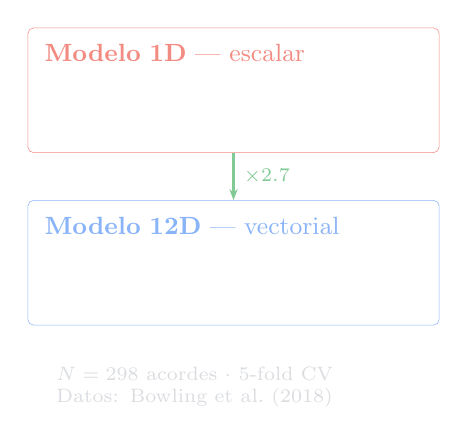
\begin{tikzpicture}[
      node distance=0.6cm,
      every node/.style={font=\small},
      metricbox/.style={
        rounded corners=2pt, 
        draw=linegray, very thin,
        text=fgwhite, 
        inner sep=6pt,
        text width=4.8cm,
        align=left
      }
    ]
      \node[metricbox, draw=accent2] (m1d) {
        {\color{accent2}\textbf{Modelo 1D} — escalar}\\[3pt]
        $r_{\mathrm{OOS}} = 0.468$\\
        $R^2_{\mathrm{OOS}} = 0.218$
      };
      \node[metricbox, draw=accent1, below=of m1d] (m12d) {
        {\color{accent1}\textbf{Modelo 12D} — vectorial}\\[3pt]
        $r_{\mathrm{OOS}} = 0.767$\\
        $R^2_{\mathrm{OOS}} = 0.588$
      };
      \draw[-{Stealth[length=4pt]}, accent3, thick] 
        (m1d.south) -- node[right, font=\scriptsize, text=accent3] {$\times 2.7$} (m12d.north);
      \node[below=0.4cm of m12d, font=\scriptsize, text=dimtext, text width=4.5cm, align=left] {
        $N=298$ acordes $\cdot$ 5-fold CV\\
        Datos: Bowling et al.\ (2018)
      };
    \end{tikzpicture}
  \end{column}
\end{columns}
\end{frame}

% ---- SLIDE 2: CONSISTENCIA ESTRUCTURAL ----
\begin{frame}{Consistencia estructural musical}
\begin{columns}[T]
  \begin{column}{0.52\textwidth}
    \vspace{0.3cm}
    \includegraphics[width=\textwidth]{triadas_conocidas.png}
  \end{column}
  \begin{column}{0.45\textwidth}
    \vspace{0.6cm}
    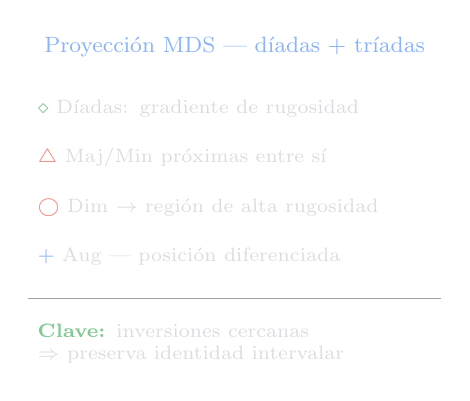
\begin{tikzpicture}[
      every node/.style={font=\small, text=fgwhite},
      obs/.style={font=\scriptsize, text=dimtext, text width=5cm, align=left}
    ]
      \node[font=\footnotesize, text=accent1] (title) {Proyección MDS — díadas + tríadas};
      \node[obs, below=0.3cm of title] (o1) {
        {\color{accent3}$\diamond$} Díadas: gradiente de rugosidad
      };
      \node[obs, below=0.15cm of o1] (o2) {
        {\color{accent2}$\triangle$} Maj/Min próximas entre sí
      };
      \node[obs, below=0.15cm of o2] (o3) {
        {\color{accent2}$\bigcirc$} Dim $\to$ región de alta rugosidad
      };
      \node[obs, below=0.15cm of o3] (o4) {
        {\color{accent1}$+$} Aug — posición diferenciada
      };
      \draw[linegray, very thin] 
        ([yshift=-0.3cm]o4.south west) -- ([yshift=-0.3cm]o4.south east);
      \node[obs, below=0.5cm of o4] (key) {
        {\color{accent3}\textbf{Clave:}} inversiones cercanas\\
        $\Rightarrow$ preserva identidad intervalar
      };
    \end{tikzpicture}
  \end{column}
\end{columns}
\end{frame}

% ---- SLIDE 3: ROBUSTEZ — TRANSPOSICIÓN Y REGISTRO ----
\begin{frame}{Robustez: transposición y registro}
\begin{columns}[T]
  \begin{column}{0.55\textwidth}
    \vspace{0.2cm}
    \includegraphics[width=\textwidth]{triadas_basicas_conregistro.jpeg}
  \end{column}
  \begin{column}{0.42\textwidth}
    \vspace{0.6cm}
    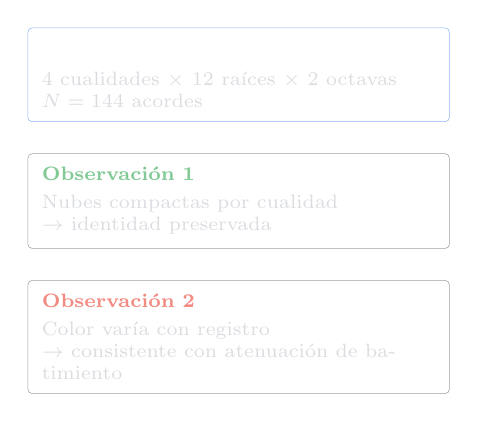
\begin{tikzpicture}[
      every node/.style={font=\footnotesize, text=fgwhite},
      param/.style={
        rounded corners=1.5pt,
        draw=linegray, very thin,
        inner sep=5pt,
        text width=5cm,
        align=left,
        font=\scriptsize,
        text=dimtext
      }
    ]
      \node[param, draw=accent1] (p) {
        {\color{fgwhite}\textbf{Diseño experimental}}\\[3pt]
        $4$ cualidades $\times$ $12$ raíces $\times$ 2 octavas\\
        $N = 144$ acordes
      };
      \node[param, below=0.4cm of p] (r1) {
        {\color{accent3}\textbf{Observación 1}}\\[2pt]
        Nubes compactas por cualidad\\
        $\to$ identidad preservada
      };
      \node[param, below=0.4cm of r1] (r2) {
        {\color{accent2}\textbf{Observación 2}}\\[2pt]
        Color varía con registro\\
        $\to$ consistente con atenuación de batimiento
      };
    \end{tikzpicture}
  \end{column}
\end{columns}
\end{frame}

% ---- SLIDE 4: ESPACIO AMPLIADO ----
\begin{frame}{Espacios armónicos ampliados}
\begin{columns}[T]
  \begin{column}{0.50\textwidth}
    \vspace{0.3cm}
    \includegraphics[width=\textwidth]{extension_triadas_conocidas.jpeg}
  \end{column}
  \begin{column}{0.47\textwidth}
    \vspace{0.5cm}
    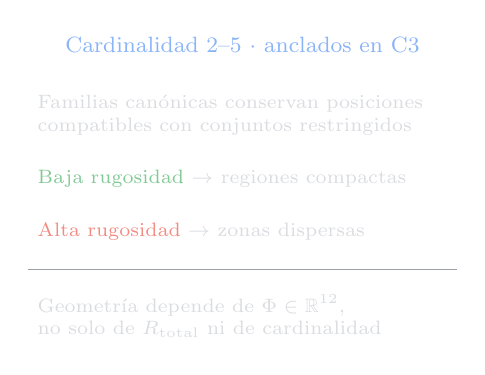
\begin{tikzpicture}[
      every node/.style={font=\small, text=fgwhite},
      block/.style={
        font=\scriptsize,
        text=dimtext,
        text width=5.2cm,
        align=left
      }
    ]
      \node[font=\footnotesize, text=accent1] (t) {
        Cardinalidad 2–5 $\cdot$ anclados en C3
      };
      \node[block, below=0.3cm of t] (b1) {
        Familias canónicas conservan posiciones\\
        compatibles con conjuntos restringidos
      };
      \node[block, below=0.2cm of b1] (b2) {
        {\color{accent3}Baja rugosidad} $\to$ regiones compactas
      };
      \node[block, below=0.2cm of b2] (b3) {
        {\color{accent2}Alta rugosidad} $\to$ zonas dispersas
      };
      \draw[linegray, very thin] 
        ([yshift=-0.25cm]b3.south west) -- ([yshift=-0.25cm]b3.south east);
      \node[block, below=0.45cm of b3] (b4) {
        Geometría depende de $\Phi \in \mathbb{R}^{12}$,\\
        no solo de $R_{\mathrm{total}}$ ni de cardinalidad
      };
    \end{tikzpicture}
  \end{column}
\end{columns}
\end{frame}

% ---- SLIDE 5: MASA ALEATORIA ----
\begin{frame}{Coherencia geométrica: masa aleatoria}
\begin{columns}[T]
  \begin{column}{0.48\textwidth}
    \vspace{0.2cm}
    \includegraphics[width=\textwidth]{masa_aleatoria.png}
  \end{column}
  \begin{column}{0.49\textwidth}
    \vspace{0.4cm}
    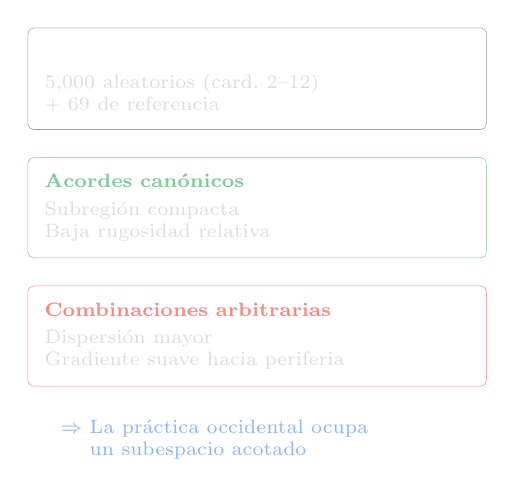
\begin{tikzpicture}[
      every node/.style={font=\small, text=fgwhite},
      box/.style={
        rounded corners=2pt,
        draw=linegray, very thin,
        inner sep=6pt,
        text width=5.4cm,
        align=left,
        font=\scriptsize,
        text=dimtext
      }
    ]
      \node[box] (n1) {
        {\color{fgwhite}\textbf{$N = 5{,}069$ acordes}}\\[3pt]
        $5{,}000$ aleatorios (card.\ 2–12)\\
        $+\;69$ de referencia
      };
      \node[box, below=0.35cm of n1, draw=accent3] (n2) {
        {\color{accent3}\textbf{Acordes canónicos}}\\[2pt]
        Subregión compacta\\
        Baja rugosidad relativa
      };
      \node[box, below=0.35cm of n2, draw=accent2] (n3) {
        {\color{accent2}\textbf{Combinaciones arbitrarias}}\\[2pt]
        Dispersión mayor\\
        Gradiente suave hacia periferia
      };
      \node[font=\scriptsize, text=accent1, below=0.3cm of n3, text width=5cm, align=left] {
        $\Rightarrow$ La práctica occidental ocupa\\
        \phantom{$\Rightarrow$ }un subespacio acotado
      };
    \end{tikzpicture}
  \end{column}
\end{columns}
\end{frame}

% ---- SLIDE 6: MÉTRICAS DE CALIDAD ----
\begin{frame}{Métricas de calidad del embedding}
\vspace{0.3cm}
\begin{columns}[T]
  \begin{column}{0.48\textwidth}
    \centering
    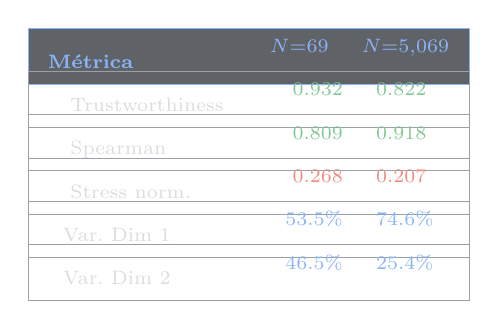
\begin{tikzpicture}[
      every node/.style={font=\footnotesize, text=fgwhite}
    ]
      % Tabla estilizada con TikZ
      \def\rw{5.6cm}
      \def\rh{0.55cm}
      
      % Header
      \node[minimum width=\rw, minimum height=\rh, 
            fill=bgdark, draw=accent1, very thin,
            font=\scriptsize\bfseries] (h) at (0,0) {
        \begin{tabular}{@{}p{2.4cm}cc@{}}
          \color{accent1}Métrica & \color{accent1}$N{=}69$ & \color{accent1}$N{=}5{,}069$
        \end{tabular}
      };
      
      % Rows
      \foreach \metric/\va/\vb/\clr [count=\i] in {
        Trustworthiness/0.932/0.822/accent3,
        Spearman/0.809/0.918/accent3,
        Stress norm./0.268/0.207/accent2,
        Var.\ Dim 1/53.5\%/74.6\%/accent1,
        Var.\ Dim 2/46.5\%/25.4\%/accent1%
      }{
        \node[minimum width=\rw, minimum height=\rh,
              draw=linegray, very thin,
              font=\scriptsize] (r\i) at (0, -\i*0.55) {
          \begin{tabular}{@{}p{2.4cm}cc@{}}
            \color{dimtext}\metric & \color{\clr}\va & \color{\clr}\vb
          \end{tabular}
        };
      }
    \end{tikzpicture}
  \end{column}
  \begin{column}{0.49\textwidth}
    \vspace{0.5cm}
    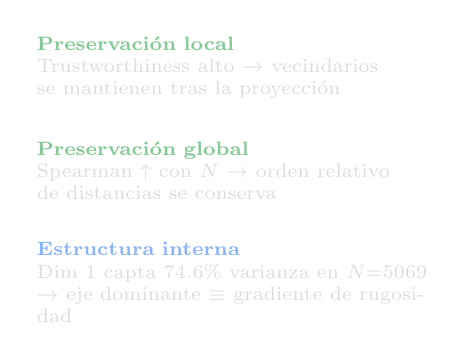
\begin{tikzpicture}[
      every node/.style={font=\scriptsize, text=dimtext, text width=5cm, align=left}
    ]
      \node (i1) {
        {\color{accent3}\textbf{Preservación local}}\\
        Trustworthiness alto $\to$ vecindarios\\
        se mantienen tras la proyección
      };
      \node[below=0.3cm of i1] (i2) {
        {\color{accent3}\textbf{Preservación global}}\\
        Spearman $\uparrow$ con $N$ $\to$ orden relativo\\
        de distancias se conserva
      };
      \node[below=0.3cm of i2] (i3) {
        {\color{accent1}\textbf{Estructura interna}}\\
        Dim 1 capta $74.6\%$ varianza en $N{=}5069$\\
        $\to$ eje dominante $\equiv$ gradiente de rugosidad
      };
    \end{tikzpicture}
  \end{column}
\end{columns}
\end{frame}

% ---- SLIDE 7: APLICACIÓN — SUSTITUCIÓN ----
\begin{frame}{Aplicación: sustitución por proximidad métrica}
\vspace{0.2cm}
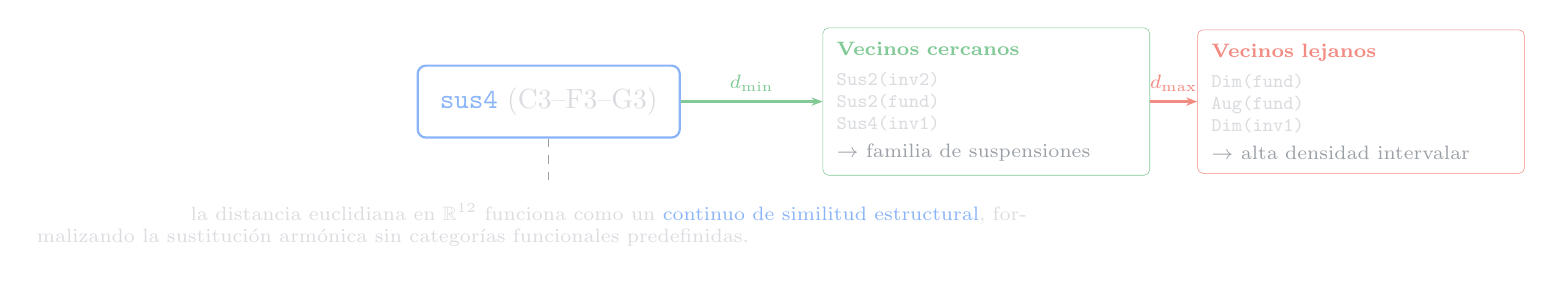
\begin{tikzpicture}[remember picture,
  every node/.style={font=\small, text=fgwhite},
  querybox/.style={
    rounded corners=3pt,
    draw=accent1, thick,
    inner sep=8pt,
    font=\normalsize
  },
  nearbox/.style={
    rounded corners=2pt,
    draw=accent3, very thin,
    inner sep=5pt,
    font=\scriptsize,
    text=dimtext,
    text width=3.8cm,
    align=left
  },
  farbox/.style={
    rounded corners=2pt,
    draw=accent2, very thin,
    inner sep=5pt,
    font=\scriptsize,
    text=dimtext,
    text width=3.8cm,
    align=left
  }
]
  % Acorde consulta
  \node[querybox] (q) at (0,0) {
    {\color{accent1}\texttt{sus4}} {\color{dimtext}(C3–F3–G3)}
  };
  
  % Vecinos cercanos
  \node[nearbox, right=1.8cm of q] (near) {
    {\color{accent3}\textbf{Vecinos cercanos}}\\[3pt]
    \texttt{Sus2(inv2)}\\
    \texttt{Sus2(fund)}\\
    \texttt{Sus4(inv1)}\\[2pt]
    {\color{linegray}$\to$ familia de suspensiones}
  };
  
  % Vecinos lejanos
  \node[farbox, right=0.6cm of near] (far) {
    {\color{accent2}\textbf{Vecinos lejanos}}\\[3pt]
    \texttt{Dim(fund)}\\
    \texttt{Aug(fund)}\\
    \texttt{Dim(inv1)}\\[2pt]
    {\color{linegray}$\to$ alta densidad intervalar}
  };
  
  % Flechas
  \draw[-{Stealth[length=4pt]}, accent3, thick] 
    (q.east) -- node[above, font=\scriptsize, text=accent3] {$d_{\min}$} (near.west);
  \draw[-{Stealth[length=4pt]}, accent2, thick] 
    (near.east) -- node[above, font=\scriptsize, text=accent2] {$d_{\max}$} (far.west);
  
  % Interpretación
  \node[below=0.7cm of q, text width=13cm, align=left, font=\scriptsize, text=dimtext] (int) {
    {\color{fgwhite}Interpretación:} la distancia euclidiana en $\mathbb{R}^{12}$ funciona como un 
    {\color{accent1}continuo de similitud estructural}, formalizando la sustitución armónica sin categorías funcionales predefinidas.
  };
  
  % Líneas conectoras
  \draw[linegray, very thin, dashed] (q.south) -- ([yshift=0.15cm]int.north -| q);
\end{tikzpicture}
\end{frame}

% ---- SLIDE 8: CIERRE ----
\begin{frame}[plain]
\begin{tikzpicture}[remember picture, overlay]
  % línea superior
  \draw[accent1, thin] 
    ([xshift=2cm, yshift=-2cm]current page.north west) -- 
    ([xshift=8cm, yshift=-2cm]current page.north west);
  
  % Resumen visual
  \node[anchor=west, text width=13cm] at 
    ([xshift=2cm, yshift=1cm]current page.west) {
      {\Large\bfseries\color{fgwhite}Síntesis de resultados}\\[12pt]
      \begin{tikzpicture}[
        node distance=0.08cm and 0.4cm,
        res/.style={
          rounded corners=2pt,
          draw=linegray, very thin,
          inner sep=5pt,
          font=\scriptsize,
          text=dimtext,
          text width=6.5cm,
          align=left
        }
      ]
        \node[res] (r1) {
          {\color{accent1}1.} Modelo 12D explica {\color{accent3}59\%} de la varianza perceptual ($R^2_{\mathrm{OOS}}$)
        };
        \node[res, below=of r1] (r2) {
          {\color{accent1}2.} Geometría MDS coherente con cualidades armónicas conocidas
        };
        \node[res, below=of r2] (r3) {
          {\color{accent1}3.} Representación robusta bajo transposición y variación de registro
        };
        \node[res, below=of r3] (r4) {
          {\color{accent1}4.} Acordes occidentales $\subset$ subregión compacta de baja rugosidad
        };
        \node[res, below=of r4] (r5) {
          {\color{accent1}5.} Sustitución armónica formalizada como proximidad en $\mathbb{R}^{12}$
        };
      \end{tikzpicture}
    };
  
  % línea inferior
  \draw[linegray, very thin] 
    ([xshift=2cm, yshift=1.2cm]current page.south west) -- 
    ([xshift=14cm, yshift=1.2cm]current page.south west);
\end{tikzpicture}
\end{frame}

\end{document}
